%!TEX root = main.tex

% \newpage


% \vspace*{\fill}
% \begin{center}
	% \section{Appendix}
% \end{center}
% \vspace*{\fill}

\newpage
\appendix
\begin{landscape}
\global\pdfpageattr\expandafter{\the\pdfpageattr/Rotate 90}
% \section{Appendix}
\section{Gantt diagrams} \label{App:A}

% \begin{figure}[!ht]
% \begin{center}
% \caption{\small \sl First semester gantt.\label{fig:gantt1}}
% \end{center}
% \end{figure}

\begin{figure}[!ht]
\begin{center}
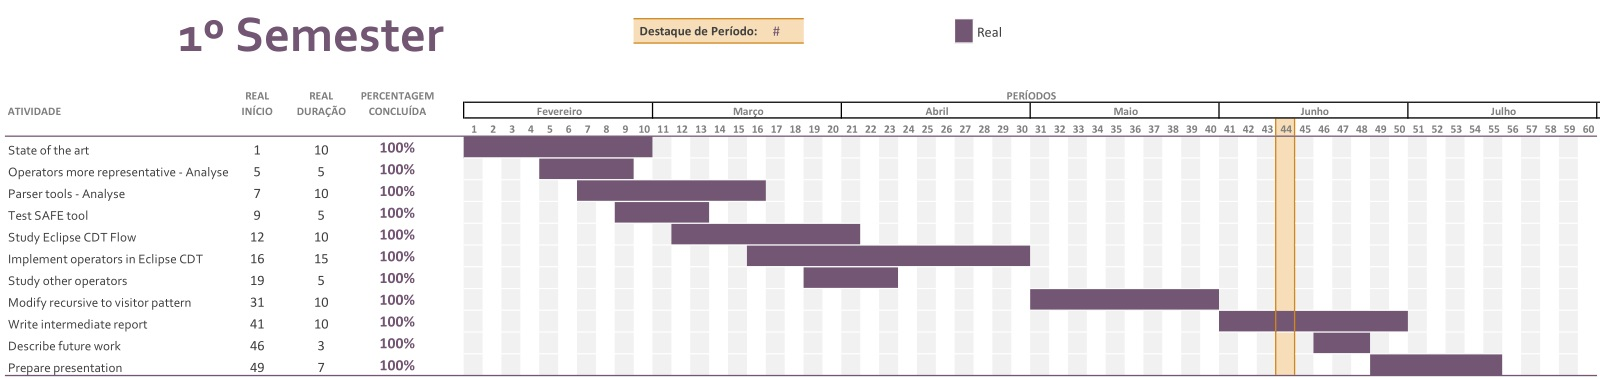
\includegraphics[width=1.5\textwidth]{gantt1.jpg}
\newline
\newline
\newline
\newline
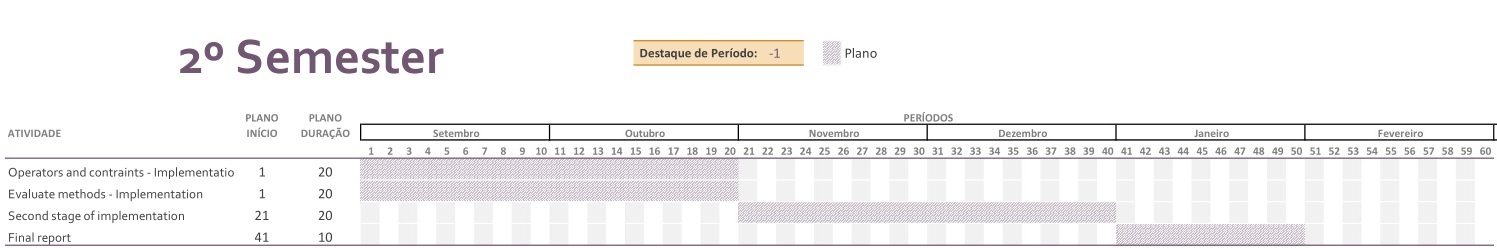
\includegraphics[width=1.5\textwidth]{gantt2.jpg}
\caption{\small \sl First and second semesters Gantt.\label{fig:gantt}}
\end{center}
\end{figure}

\clearpage

\section{Risks table} \label{App:B}
\begin{figure}[!ht]
\begin{center}
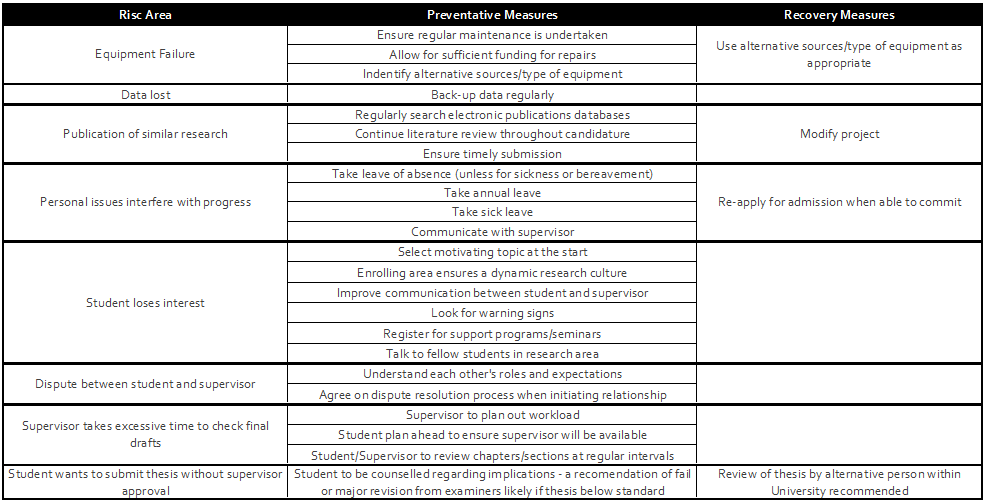
\includegraphics[width=1.5\textwidth]{risks.png}
\caption[\small \sl Risks]{\small \sl Risks (Adapted from Managing Your Thesis: a Quick Reference Guide by Curtin University
\cite{_gs_managing_thesis}).
\label{fig:risks}}
\end{center}
\end{figure}

\end{landscape}
\global\pdfpageattr\expandafter{\the\pdfpageattr/Rotate 0}

\clearpage
% \printacronyms[include-classes=abbrev,name={\section{Abbreviations} \label{App:C}}]
% \iftoggle{long}{\acuseall}

% \printacronyms[include-classes=operator,name=Operators]
% \printacronyms[include-classes=constraint,name=Constraints]
